\documentclass[preview]{standalone}
\usepackage{tikz}
\usetikzlibrary{mindmap}

\begin{document}
\tikzstyle{branch}=[fill,shape=circle,minimum size=3pt,inner sep=0pt]
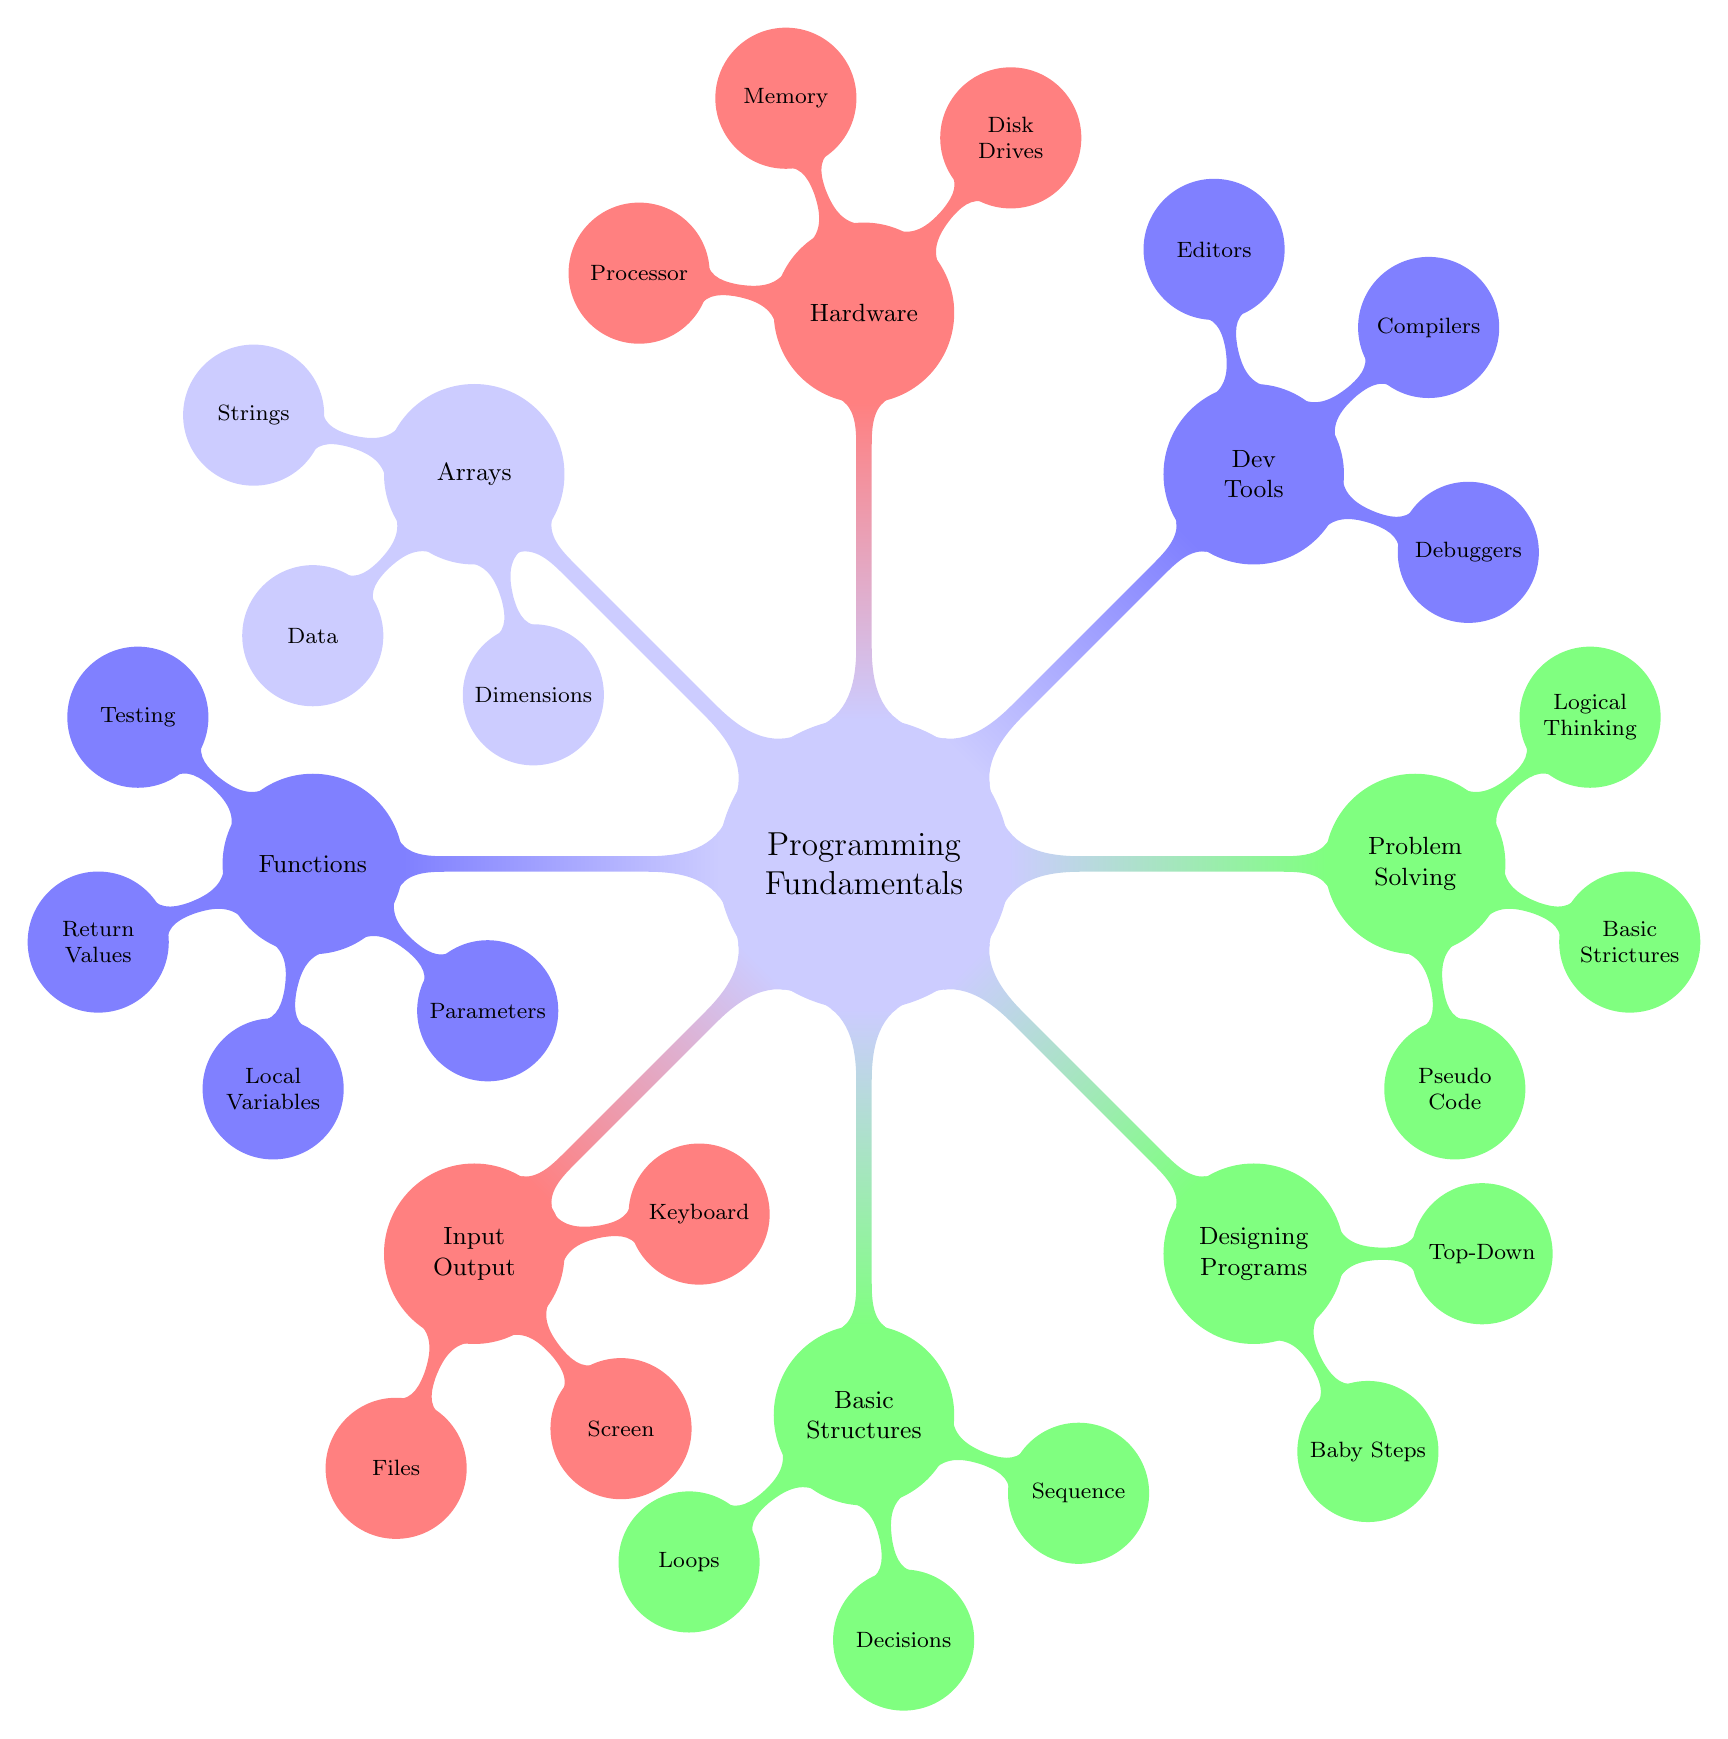
\begin{tikzpicture}
[root concept/.append style={concept color=blue!20, minimum size=2cm},
    level 1 concept/.append style={level distance=7cm, sibling angle=45},
    mindmap]
\node [concept] {Programming\\Fundamentals}
    [clockwise from=90]
    child [concept color=red!50] {node [concept] {Hardware}
        [clockwise from=170]
        child {node [concept] {Processor} }
        child {node [concept] {Memory} }
        child {node [concept] {Disk Drives} }
    }
    child [concept color=blue!50] {node [concept] {Dev\\Tools}
        [clockwise from=100]
        child {node [concept] {Editors} }
        child {node [concept] {Compilers} }
        child {node [concept] {Debuggers} }
    }
    child [concept color=green!50] {node [concept] {Problem\\Solving}
        [clockwise from=40]
        child {node [concept] {Logical\\Thinking} }
        child {node [concept] {Basic\\Strictures} }
        child {node [concept] {Pseudo\\Code} }
    }
    child [concept color=green!50] {node [concept] {Designing\\Programs}
        [clockwise from=0]
        child {node [concept] {Top-Down} }
        child {node [concept] {Baby Steps} }
    }
    child [concept color=green!50] {node [concept] {Basic\\Structures}
       [clockwise from=-20]
       child {node [concept] {Sequence} }
       child {node [concept] {Decisions} }
       child {node [concept] {Loops} }
    }
    child [concept color=red!50] {node [concept] {Input\\Output}
        [clockwise from=10]
        child {node [concept] {Keyboard} }
        child {node [concept] {Screen} }
        child {node [concept] {Files} }
    }
    child [concept color=blue!50] {node [concept] {Functions}
        [clockwise from=-40]
        child {node [concept] {Parameters} }
        child {node [concept] {Local\\Variables} }
        child {node [concept] {Return\\Values} }
        child {node [concept] {Testing} }
    }
    child [concept] {node [concept] {Arrays}
        [clockwise from=-75]
        child {node [concept] {Dimensions} }
        child {node [concept] {Data} }
        child {node [concept] {Strings} }
    };
\end{tikzpicture}
\end{document}
